\subsection{Terzaghi consolidation: Monolithic and staggered approaches}

In the HM problem, mechanical compression generates a fluid pressure response, while pressure storage and dissipation affect the mechanical condition via the effective stress. Terzaghi has provided the framework to test such a problem. A cartoon of the problem to be examined is shown in Fig. \ref{terz:cartoon}. This test is a necessary, but not fully sufficient condition for correct implementation of a hydromechanical simulator. It guarantees correct implementation of the coupling relationships between the 1)fluid and 2)mechanical system.

\begin{figure}[!tbh]
\begin{center}
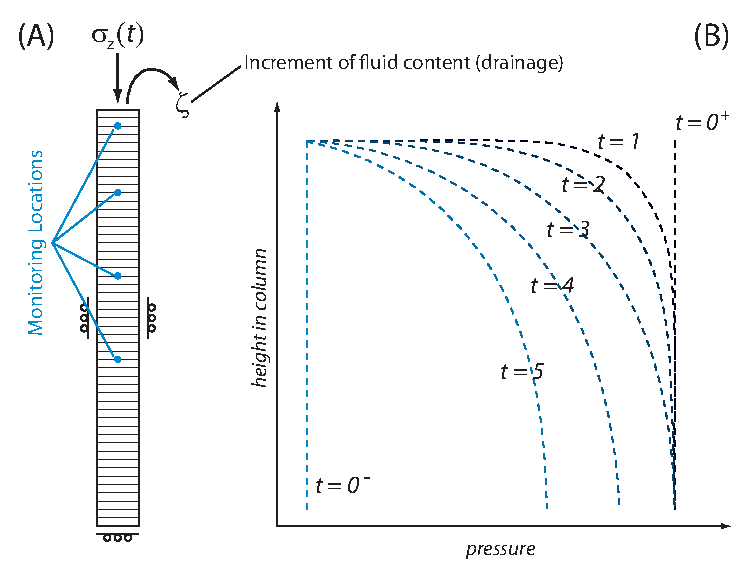
\includegraphics[width=0.7\textwidth]{chapter_14/figures/fig_14_1_1}
\end{center}
\caption{Terzaghi problem. A.) 2-D column ($p=0$ initially) stress applied to top of column which is a free draining boundary. Other boundaries are no-flow and roller displacement. Stress may be applied as a single step-load, or as a function of time. Pressure and displacement are monitored in time at specific locations. B.) Anticipated (conceptual) pressure profiles within the column with the progression of time for a step-load of applied stress (in full column, not at monitoring locations).}
\label{terz:cartoon}
\end{figure}

\subsubsection*{Definition}
For a single fluid phase, the analytical solution for pressure dissipation is available.  The analytical solution to this problem has been utilized a number of times for this very purpose. Beginning from the 1-D fluid diffusion equation of hydrogeology (simply a fluid mass balance equation),

\begin{equation}
\frac{\partial p}{\partial t}-c\frac{{{\partial }^{2}}p}{\partial {{z}^{2}}}=0,
\end{equation}

where $c$ is 1-D fluid diffusivity.  The pore pressure response to a vertical load, $\sigma _{z}$, applied linearly over time ($\sigma _{z}^{t={{0}^{-}}}=0$) to the top of the column at a rate, ${{\dot{\sigma }}_{z}}=d{{\sigma }_{z}}/dt$, is, (\cite{Wang:00}, Eq. 6.50),

\begin{equation}
\begin{split}
\frac{p\left( z,t \right)}{{{p}_{0}}}=\left\{ 1-{{\left( \frac{L-z}{L} \right)}^{2}}-\right.\left. \frac{32}{{{\pi }^{3}}}\left[ \sum\limits_{m=0}^{\infty }{\frac{{{\left( -1 \right)}^{m}}}{{{\left( 2m+1 \right)}^{3}}}\exp \left[ -{{\psi }^{2}}ct \right]\cos \left[ \psi \left( L-z \right) \right]} \right] \right\},
\end{split}
\end{equation}

where the total pressure generation is

\begin{equation}
{{p}_{0}}=\frac{{{L}^{2}}}{2c}\left( {{B}_{v}}{{{\dot{\sigma }}}_{z}} \right),
\end{equation}

for the factor, $\psi =\left( 2m+1 \right)\pi /\left( 2L \right)$, the total column length, $L$, and the location in the column (downward from the applied stress), $z$. The 1-D Skempton coefficient,

\begin{equation}
{{B}_{v}}={{\left. -\frac{\delta \bar{p}}{\delta {{\sigma }_{zz}}} \right|}_{{{\varepsilon }_{xx}}={{\varepsilon }_{yy}}=\zeta =0}}=\frac{\alpha }{{{K}_{v}}{{S}_{v}}},
\end{equation}

is given purely by micromechanical, poroelastic considerations from the uniaxial drained bulk modulus, $K_{v}$, and the 1-D specific storage, $S_{v}$ (Table \ref{terz:tab1}). The 1-D diffusivity is also a derivative of the 1-D storage:

\begin{equation}
c=\frac{k}{\mu {{S}_{v}}},
\end{equation}

and also the permeability, $k$, and viscosity, $\mu$. See Table \ref{terz:tab1}, \cite{DetournayCheng:93}, and \cite{Wang:00} for additional details regarding poroelastic relationships. If utilizing an applied step load at time $t={{0}^{+}}$ we can generate another analytical solution for pressure, and also displacement. For this validation, we utilize only the linear loading rate. Because displacement is the primary variable in our FEM formulation, the displacement must be accurate in order to generate the correct pressure response: we find no need to reproduce the results of a step load analysis here.

\begin{table}[!htb]
\begin{center}
\begin{tabular}{lll}
\hline\noalign{\smallskip}
Parameter & Description & Equation \\
\noalign{\smallskip}\hline\noalign{\smallskip}
$B$         & Skempton coefficient & ${\alpha }/{\left[ \alpha -\phi \left( 1-\alpha  \right)+\phi K/{{K}_{f}} \right]}\;$ \\
$K^{u}$     & Undrained bulk modulus & $K/\left( 1-\alpha B \right)$ \\
$G$         & Shear modulus & $3K\left( 1-2\nu  \right)/\left( 2+2\nu  \right)$ \\
$\nu ^{u}$  & Undrained Poisson's ratio &  ${\left( 3{{K}^{u}}-2G \right)}/{\left( 6{{K}^{u}}+2G \right)}\;$ \\
$B_{v}$     & Uniaxial Skempton coefficient &  $B{\left( 1+{{\nu }_{u}} \right)}/{\left( 3-3{{\nu }_{u}} \right)}\;$ \\
$K_{v}$     & Uniaxial bulk modulus & $3K{\left( 1-\nu  \right)}/{\left( 1+\nu  \right)}\;$ \\
$K_{v}^{u}$ & Uniaxial undrained bulk modulus & ${3{{K}^{u}}\left( 1-{{\nu }^{u}} \right)}/{\left( 1+{{\nu }^{u}} \right)}\;$ \\
$S_{v}$     & Uniaxial storage & ${\alpha }/{\left( {{K}_{v}}{{B}_{v}} \right)}\;$ \\
\noalign{\smallskip}\hline
\end{tabular}
\end{center}
\caption{Fundamental poroelastic relationships. Many potential combinations are available, these representing only one possibility.}
\label{terz:tab1}
\end{table}

We choose a rather long (50m) column of rock with material properties similar to those of Berea sandstone (Table \ref{terz:tab2}).  The column is discretized uniformly into 50 FEM grid cells. Geometry is shown in Fig. \ref{terz:cartoon}, which shows a single column surrounding by displacement roller boundaries allowed to compress from the top where a loading rate, ${{\dot{\sigma }}_{z}}$, is applied at time $t=0^{+}$. Fluid pressure is initially null. Compression of the column leads to a rapid pressure increase and a subsequent drainage of pressure over time from the top of the column. The load is applied quickly enough to allow pressure to build with time. The topmost boundary is free drainage for fluid flow, all others being no-flow.

\begin{table}[!htb]
\begin{center}
\begin{tabular}{lccl}
\hline\noalign{\smallskip}
Property & Symbol & Unit & Value \\
\noalign{\smallskip}\hline\noalign{\smallskip}
\textit{Berea sandstone} & & & \\
Drained bulk modulus & $K$ & $GPa$ & 8.0 \\
Poisson ratio & $\nu $ & $-$ & 0.20 \\
Porosity & $\phi $ & $-$ & 0.19 \\
Permeability & $k$ & $m^{2}$ & $1.9\times 10^{-13}$ \\
Biot-Willis coefficient & $\alpha $ & $-$ & 0.8 \\
 & & & \\
\textit{Westerly granite} & & & \\
Drained bulk modulus & $K$ & $GPa$ & 25.0 \\
Poisson ratio & $\nu $ & $-$ & 0.25 \\
Porosity & $\phi $ & $-$ & 0.02 \\
Permeability & $k$ & $m^{2}$ & $5.0\times 10^{-15}$ \\
Biot-Willis coefficient & $\alpha $ & $-$ & 0.6 \\
\noalign{\smallskip}\hline
\end{tabular}
\end{center}
\caption{Solid properties.}
\label{terz:tab2}
\end{table}

\begin{table}[!htb]
\begin{center}
\begin{tabular}{lccc}
\hline\noalign{\smallskip}
Property & Symbol & Unit & Value \\
\noalign{\smallskip}\hline\noalign{\smallskip}
Bulk modulus   & $K_{f}$      & $GPa$         & $2.27$ \\
Density        & $\rho $      & $kg/m^3$      & $997.05$ \\
Viscosity      & $\mu $       & $Pa\times s$    & $8.9008\times 10^{-4}$ \\
\noalign{\smallskip}\hline
\end{tabular}
\end{center}
\caption{Fluid properties.}
\label{terz:tab3}
\end{table}

\subsubsection*{Results}

Simulations are conducted using both a staggered (fluid and solid equations solved iteratively) and monolithic (fluid and solid equations solved in a single matrix) with OpenGeoSys. Results are shown in Fig. \ref{terz:res1} for two alternate material property scenarios: Berea sandstone and Westerly granite. The solution is accurate in all cases. We note a small inaccuracy in the slower loading rate for sandstone that illustrates the impact of tolerance in the time step control. Here, we add one extra data set (small dots) with tighter time control, which shows that tighter accuracy can be achieved with this adjustment.

\begin{figure}[!tbh]
\begin{center}
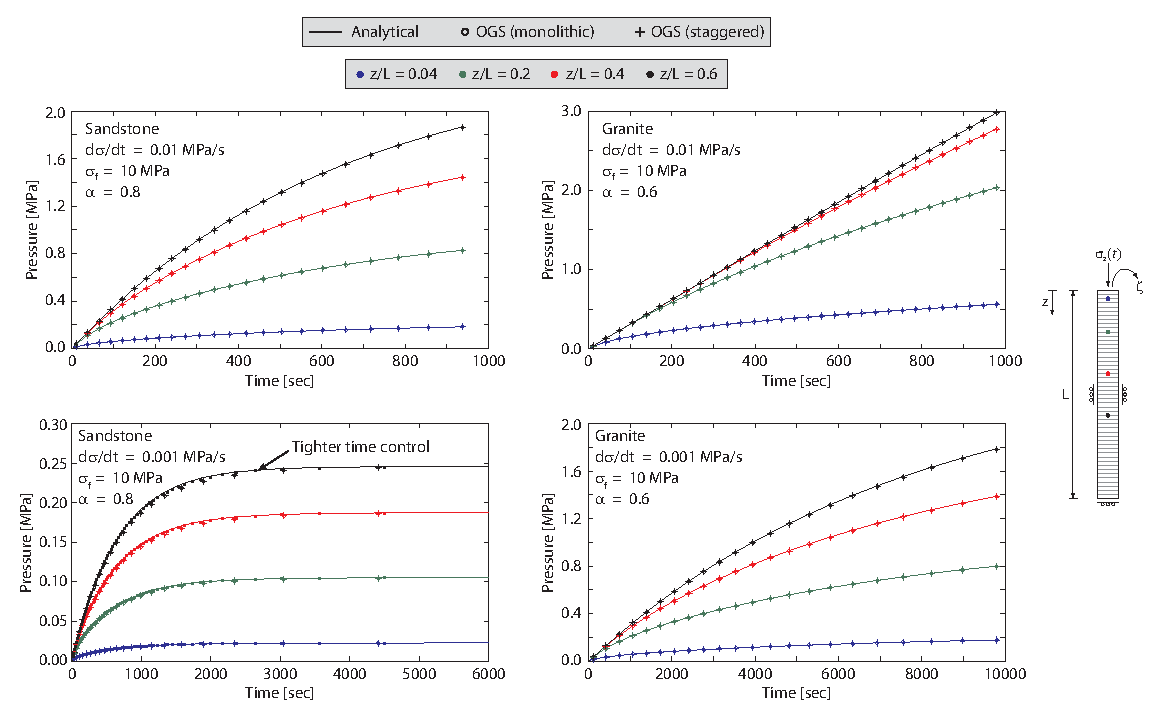
\includegraphics[width=1.0\textwidth]{chapter_14/figures/fig_14_1_2}
\end{center}
\caption{Results of HM coupling.}
\label{terz:res1}
\end{figure}

While the monolithic solution is unconditionally stable for an implicit time-stepping scheme, the staggered solution suffers limitations. When the fluid becomes highly incompressible relative to the solid, the solution will diverge. We provide the general criterion that stability is achieved with $B_v<0.5$. This criterion is generally independent of loading rate. The implications of this are important, such that for Westerly granite if incompressible grains are used the solution is unstable at $25 ^{o}C$ for the properties of Table \ref{terz:tab2}. Stability can be enforced by increasing the value of porosity that is used, or decreasing $\alpha $, or with any adjustment that brings $B_v$ above 0.5. The staggered solution is stable for all realistic cases (everything compressible) we have tried. For very sharply applied loads such as a step load applied at $t=0^+$, however, the staggered solution will become unstable even with this criterion. It is important for a given problem and set of solid/fluid properties to examine stability with the above benchmark before extending to the full system.

Time steps are adaptively controlled with a tolerance based on the rate of pressure change over a time step. Such a scheme is capable of ensuring accuracy in HM or H$^2$M problems. Note the importance of the tolerance in Fig. \ref{terz:res1}.